\documentclass[journal,12pt,twocolumn]{IEEEtran}

\usepackage{setspace}
\usepackage{gensymb}
\singlespacing
\usepackage[cmex10]{amsmath}

\usepackage{amsthm}

\usepackage{mathrsfs}
\usepackage{txfonts}
\usepackage{stfloats}
\usepackage{bm}
\usepackage{cite}
\usepackage{cases}
\usepackage{subfig}

\usepackage{longtable}
\usepackage{multirow}

\usepackage{enumitem}
\usepackage{mathtools}
\usepackage{steinmetz}
\usepackage{tikz}
\usepackage{circuitikz}
\usepackage{verbatim}
\usepackage{tfrupee}
\usepackage[breaklinks=true]{hyperref}
\usepackage{graphicx}
\usepackage{tkz-euclide}

\usetikzlibrary{calc,math}
\usepackage{listings}
    \usepackage{color}                                            %%
    \usepackage{array}                                            %%
    \usepackage{longtable}                                        %%
    \usepackage{calc}                                             %%
    \usepackage{multirow}                                         %%
    \usepackage{hhline}                                           %%
    \usepackage{ifthen}                                           %%
    \usepackage{lscape}     
\usepackage{multicol}
\usepackage{chngcntr}

\DeclareMathOperator*{\Res}{Res}

\renewcommand\thesection{\arabic{section}}
\renewcommand\thesubsection{\thesection.\arabic{subsection}}
\renewcommand\thesubsubsection{\thesubsection.\arabic{subsubsection}}

\renewcommand\thesectiondis{\arabic{section}}
\renewcommand\thesubsectiondis{\thesectiondis.\arabic{subsection}}
\renewcommand\thesubsubsectiondis{\thesubsectiondis.\arabic{subsubsection}}

\newtheorem{theorem}{Theorem}
\hyphenation{op-tical net-works semi-conduc-tor}
\def\inputGnumericTable{}                                 %%

\lstset{
%language=C,
frame=single, 
breaklines=true,
columns=fullflexible
}
\begin{document}

\newcommand{\BEQA}{\begin{eqnarray}}
\newcommand{\EEQA}{\end{eqnarray}}
\newcommand{\define}{\stackrel{\triangle}{=}}
\bibliographystyle{IEEEtran}
\raggedbottom
\setlength{\parindent}{0pt}
\providecommand{\mbf}{\mathbf}
\providecommand{\pr}[1]{\ensuremath{\Pr\left(#1\right)}}
\providecommand{\qfunc}[1]{\ensuremath{Q\left(#1\right)}}
\providecommand{\sbrak}[1]{\ensuremath{{}\left[#1\right]}}
\providecommand{\lsbrak}[1]{\ensuremath{{}\left[#1\right.}}
\providecommand{\rsbrak}[1]{\ensuremath{{}\left.#1\right]}}
\providecommand{\brak}[1]{\ensuremath{\left(#1\right)}}
\providecommand{\lbrak}[1]{\ensuremath{\left(#1\right.}}
\providecommand{\rbrak}[1]{\ensuremath{\left.#1\right)}}
\providecommand{\cbrak}[1]{\ensuremath{\left\{#1\right\}}}
\providecommand{\lcbrak}[1]{\ensuremath{\left\{#1\right.}}
\providecommand{\rcbrak}[1]{\ensuremath{\left.#1\right\}}}
\theoremstyle{remark}
\newtheorem{rem}{Remark}
\newcommand{\sgn}{\mathop{\mathrm{sgn}}}
\providecommand{\abs}[1]{\vert#1\vert}
\providecommand{\res}[1]{\Res\displaylimits_{#1}} 
\providecommand{\norm}[1]{\lVert#1\rVert}
%\providecommand{\norm}[1]{\lVert#1\rVert}
\providecommand{\mtx}[1]{\mathbf{#1}}
\providecommand{\mean}[1]{E[ #1 ]}
\providecommand{\fourier}{\overset{\mathcal{F}}{ \rightleftharpoons}}
%\providecommand{\hilbert}{\overset{\mathcal{H}}{ \rightleftharpoons}}
\providecommand{\system}{\overset{\mathcal{H}}{ \longleftrightarrow}}
	%\newcommand{\solution}[2]{\textbf{Solution:}{#1}}
\newcommand{\solution}{\noindent \textbf{Solution: }}
\newcommand{\cosec}{\,\text{cosec}\,}
\providecommand{\dec}[2]{\ensuremath{\overset{#1}{\underset{#2}{\gtrless}}}}
\newcommand{\myvec}[1]{\ensuremath{\begin{pmatrix}#1\end{pmatrix}}}
\newcommand{\mydet}[1]{\ensuremath{\begin{vmatrix}#1\end{vmatrix}}}
\numberwithin{equation}{subsection}
\makeatletter
\@addtoreset{figure}{problem}
\makeatother
\let\StandardTheFigure\thefigure
\let\vec\mathbf
\renewcommand{\thefigure}{\theproblem}
\def\putbox#1#2#3{\makebox[0in][l]{\makebox[#1][l]{}\raisebox{\baselineskip}[0in][0in]{\raisebox{#2}[0in][0in]{#3}}}}
     \def\rightbox#1{\makebox[0in][r]{#1}}
     \def\centbox#1{\makebox[0in]{#1}}
     \def\topbox#1{\raisebox{-\baselineskip}[0in][0in]{#1}}
     \def\midbox#1{\raisebox{-0.5\baselineskip}[0in][0in]{#1}}
\vspace{3cm}
\title{Quiz 1}
\author{Digjoy Nandi - AI20BTECH11007}
\maketitle
\newpage
\bigskip
\renewcommand{\thefigure}{\theenumi}
\renewcommand{\thetable}{\theenumi}
Download all python codes from 
\begin{lstlisting}
https://github.com/Digjoy12/Signal-Processing/blob/main/Assignment_5/Codes/Code.py
\end{lstlisting}
%
and latex codes from 
%
\begin{lstlisting}
https://github.com/Digjoy12/Signal-Processing/blob/main/Assignment_5/main.tex
\end{lstlisting}
\section*{\textbf{Problem}}
\textbf{(Q 2.7)} Determine whether each of the following signals is periodic. If the signal is periodic, state its period.
\begin{align*}
(a) x[n] &= \exp(j(\pi n/6))\\
(b) x[n] &= \exp(j(3\pi n/4))\\
(c) x[n] &= [sin(\pi n/5)]/(\pi n)
\end{align*}
    
\section*{\textbf{Solution}}
We know that, x[n] is periodic with period N if x[n] = x[n+N] for some integer N.
\begin{enumerate}
    \item Let,
    \begin{align}
        x[n] &= x[n+N]\\
        \implies \exp{\left(\cfrac{j(\pi n)}{6}\right)} &= \exp{\left(\cfrac{j(\pi (n+N))}{6}\right)}
    \end{align}
Now,
\begin{align}
  \exp{\left(\cfrac{j(\pi (n+N))}{6}\right)} &= \exp{\left(j(\frac{\pi}{6}n + 2\pi k)\right)}\\
  \implies 2\pi k &= \cfrac{\pi}{6}N,\text{for integers k,N}\\
  \implies N &= 12k
\end{align}
Hence, for k = 1, x[n] is a \textbf{periodic function} which have a period of 12.\\
\begin{figure}[!ht]
\centering
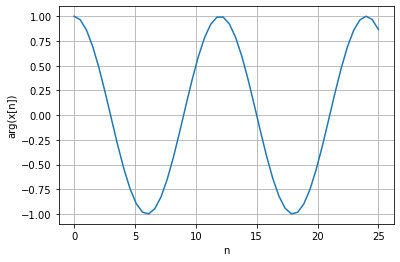
\includegraphics[width=\columnwidth]{fig_1.png}
\caption{Plot of x[n] = \exp(j(\pi n/6)) }
\end{figure}
\item
Let,
\begin{align}
    x[n] &= x[n+N]\\
    \implies \exp{j(\cfrac{3\pi n}{4})} &= \exp{j(\frac{3\pi}{4})(n+N)}
\end{align}
Now,
\begin{align}
    \exp{j(\frac{3\pi}{4})(n+N)} &= \exp{j(\frac{3\pi n}{4}+2\pi k)}\\
    \implies 2\pi k &= \cfrac{3\pi}{4}N,\text{for integers k,N}\\
    \implies N = \cfrac{8}{3}k
\end{align}
Hence, for k = 3, x[n] is a \textbf{periodic function} which have a period of 8.\\
\begin{figure}[!ht]
\centering
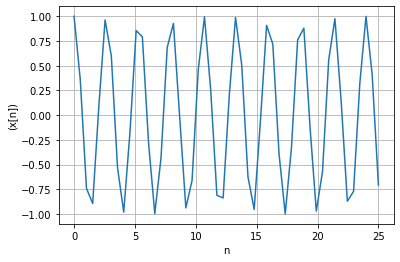
\includegraphics[width=\columnwidth]{fig_2.png}
\caption{Plot of x[n] = \exp(j(3\pi n/4)) }
\end{figure}
\item
Let,
\begin{align}
    x[n] &= x[n+N]\\
    \cfrac{[sin(\pi n/5)]}{\pi n} &= \cfrac{[sin(\pi(n+N)]}{\pi(n+N)}\\
                                 &= \cfrac{[sin(\pi n/5 + N/5)]}{\pi n + \pi N}
\end{align}
Since, the denominator term is linear in n.\\
Hence, x[n] is \textbf{not a periodic function}. \\
\begin{figure}[!ht]
\centering
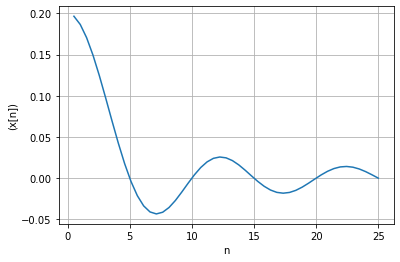
\includegraphics[width=\columnwidth]{fig_3.png}
\caption{Plot of x[n] = [sin(\pi n/5)]/(\pi n)}
\end{figure}
    
\end{enumerate}



\end{document}

